\subsection{System Architecture and Block Diagram}

The architecture of the overall system can be described as a unified hardware and software control system that has been developed by using an embedded platform. This is because the architecture uses a modular approach where sensing, decision making, and actuation have separate roles. Hence, both the baseline and reinforcement learning-based architectures share the same hardware system.

\begin{figure}[h!]
    \vspace{0.5cm} 
    \centering
    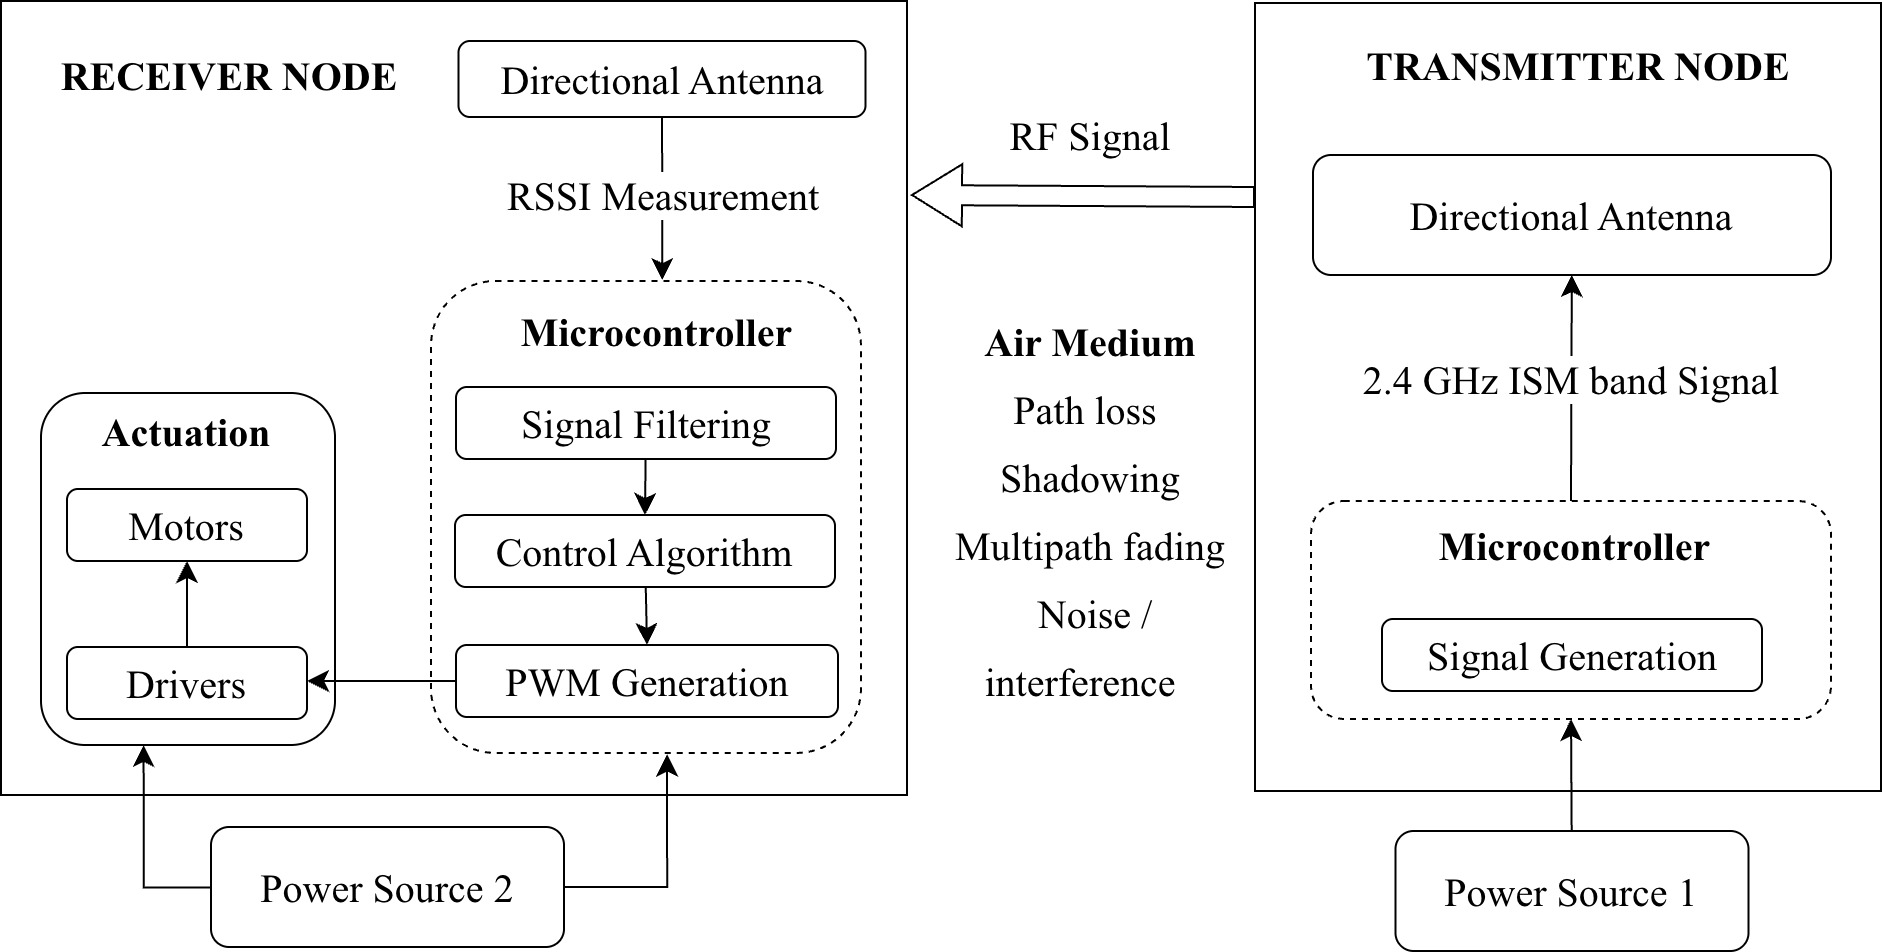
\includegraphics[width=1\textwidth]{images/system_block_diagram.jpg}
    \vspace{0.25cm}
    \caption{High-Level System Block Diagram}
    \label{fig:system_block}
\end{figure}

\subsubsection{High-Level Hardware Architecture}
A schematic diagram for the hardware architecture of the suggested system can be
seen in Figure~\ref{fig:system_block}. The ESP32-S3 microcontroller is the main
processor which performs all the processing and control operations.

The important hardware elements include:
\begin{itemize}
    \item \textbf{ESP32-S3 Microcontroller}: Performs the role of central
    controller which executes the task of acquiring RSSI, executing the control
    algorithms, performing the logging of the results and controlling actuators
    \item \textbf{Directional Antenna}: Attached to the pan-tilt mount and
    connected to the ESP32-S3 radio subsystem to receive packets from a fixed
    transmitter 
    \item \textbf{Azimuth Actuator}: A NEMA 17 stepper motor which performs the
    rotation of the antenna around the horizontal axis
    \item \textbf{Tilt Actuator}: An MG90S servo motor which controls the tilt
    angle in the vertical direction
    \item \textbf{Motor Driver (A4988)}: An interface module that allows to drive
    a stepper motor based on the digital commands from the ESP32-S3
    \item \textbf{Power Supply Unit}: Supplies regulated power to the ESP32-S3,
    the servo motor and the stepper driver, and supplies power to the stepper
    motor with a separate high-current channel
\end{itemize}

There are some differences in the implementation of azimuth and tilt motions in
the prototype device. Namely, the stepper motor and A4988 driver are used only
for azimuth motion, while the tilt motion is provided directly by the servo,
connected to the ESP32-S3 through PWM signal. The communication protocol for
stepper driver is based on GPIO pins (STEP, DIR, and ENABLE) on the ESP32-S3.
No feedback is used from any of the actuators.

\subsubsection{Software Architecture Overview}
The software architecture follows the same design philosophy of modularization found in the hardware design, and consists of four functional modules that are implemented on the ESP32:
\begin{itemize}
    \item \textbf{RSSI Reception Module}: Receives wireless packets and extracts their RSSI values through the radio system on the ESP32. A simple filter mechanism is implemented to address rapid fluctuation problems
    
    \item \textbf{State Encoding Module}: Encodes the raw RSSI measurements and the antenna's orientation angle to form a concise and discrete state for further processing in the decision process
    
    \item \textbf{Decision Module}: Implements one of the two alignment approaches depending on the chosen control algorithm (i.e., either scanning, hill-climbing or reinforcement learning)
    
    \item \textbf{Motor Action Module}: Executes the chosen action and sends appropriate control signals to the stepper motor driver module
\end{itemize}

The four modules are run sequentially within a fixed cycle time in a control loop.

\subsubsection{Data Flow and Control Loop}

Figure~\ref{fig:control_flow} illustrates the main data flow and control loop of the system. The steps involved include the following:

\begin{itemize}
    \item The MCU acquires wireless packets using the directional antenna and obtains the respective RSSI values.
    \item The filtered RSSI values are input into the state encoder unit along with the current azimuth and tilt indices.
    \item The decision maker analyzes the present state and makes a choice regarding the action based on the alignment policy being used.
    \item The antenna control unit sends the motor control signals to either move the antenna in azimuth or tilt angle.
    \item The mechanical stabilization of the antenna is ensured prior to acquiring the next set of RSSI values.
    \item The new orientation of the antenna influences the future RSSI values, thus completing the control loop.
\end{itemize}

The closed-loop process goes on until a convergence point is reached.

\begin{figure}[H]
    \vspace{1em} 
    \centering
    \includegraphics[width=1\textwidth]{images/flowdiagram.jpg}
    \vspace{0.25cm}
    \caption{System Data Flow Diagram}
    \label{fig:control_flow}
\end{figure}